\documentclass{beamer}
\usepackage[utf8]{inputenc}
\usepackage[round]{natbib}

\begin{document}

\title{Wealth Effect in Bilateral Exchange Networks}
\author{David Prentiss}
\institute{CSS695}
\date{\today}

\frame{\titlepage}

\begin{frame}
  \frametitle{Background}
  \begin{itemize}
  \item \cite{albin1992decentralized}: Agents trade two goods with partners found by
    broadcasting interests.
  \item \cite{wilhite2001bilateral}: The effects of different network
  topologies on agents engaged in bilateral trade.
  \item \cite{sunder2002simple}: An iterative scheme where traders retain
  price information from previous epochs of trading.
  \item \cite{axtell2005complexity}: Agents trading bilaterally are more
    efficient than the Walrasian process for large numbers of agents and goods.
  \item What if we used wealth effects to update trading partners iteratively?
  \item Baby duck syndrome? \(P = NP\)? Why does bilateral trade produce wealth effects?
  \end{itemize}
\end{frame}

\begin{frame}
  \frametitle{Agents}
  \begin{itemize}
  \item Trade two goods with uniformly distributed endowments \citep{albin1992decentralized}
  \item Symmetric Cobb-Douglas utility function
  \item Trades with immediate neighbors in a network
    \begin{enumerate}
    \item Check previous bid
\item Accept rational bids
  \item Make best bid to one neighbor
  \end{enumerate}
  \item Bids accepted or rejected in the following round
    \item When trading is exhausted (each epoch) allocations are reset and the
      network is updated
  \end{itemize}
\end{frame}

\begin{frame}
  \frametitle{Network}
  \begin{itemize}
  \item Initialized with ring topology
  \item Each trader has two neighbors
  \item Two network update heuristics
  \end{itemize}
\end{frame}

\begin{frame}
  \frametitle{Add-only Network Update Heuristic}
  At the end of each epoch:
  \begin{enumerate}
  \item Identify worst-off agent
  \item Add edge to next-worst-off agent that is not already a neighbor
  \item Stop when graph is complete
  \end{enumerate}
\end{frame}

\begin{frame}
  \frametitle{Add-only Network Update Heuristic}
  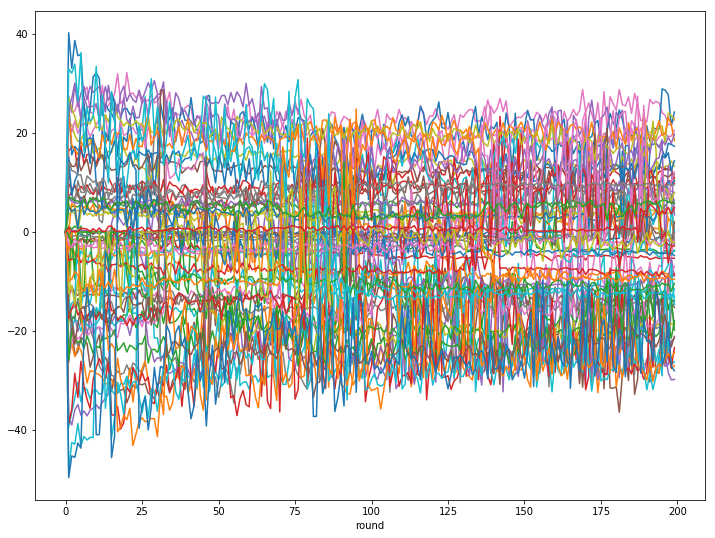
\includegraphics[width=\textwidth]{h1startwealth.png}
\end{frame}

\begin{frame}
  \frametitle{Add-only Network Update Heuristic}
  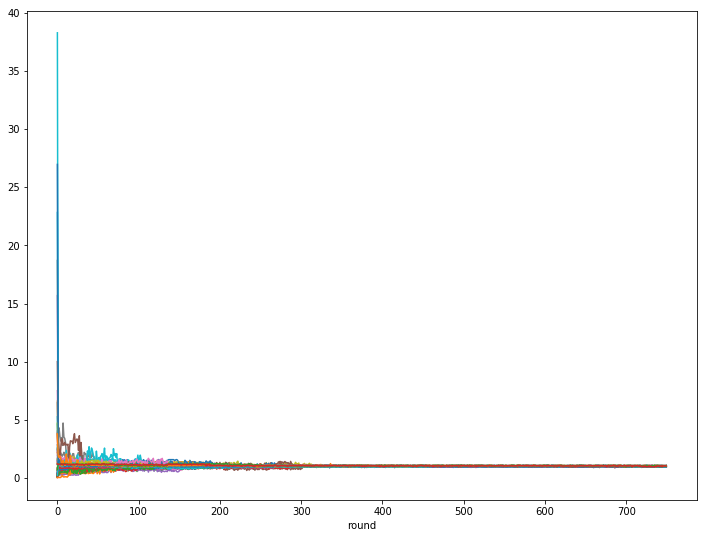
\includegraphics[width=\textwidth]{h1prices.png}
\end{frame}

\begin{frame}
  \frametitle{Add-only Network Update Heuristic}
  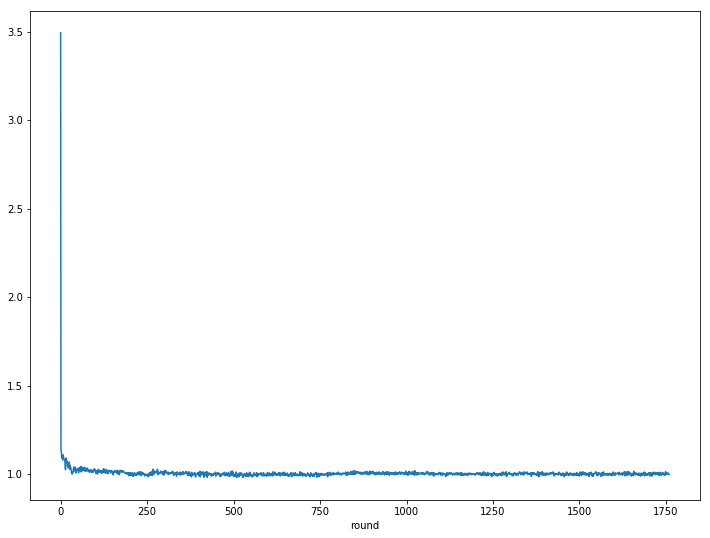
\includegraphics[width=\textwidth]{h1allpriceave.png}
\end{frame}

\begin{frame}
  \frametitle{Add-only Network Update Heuristic}
  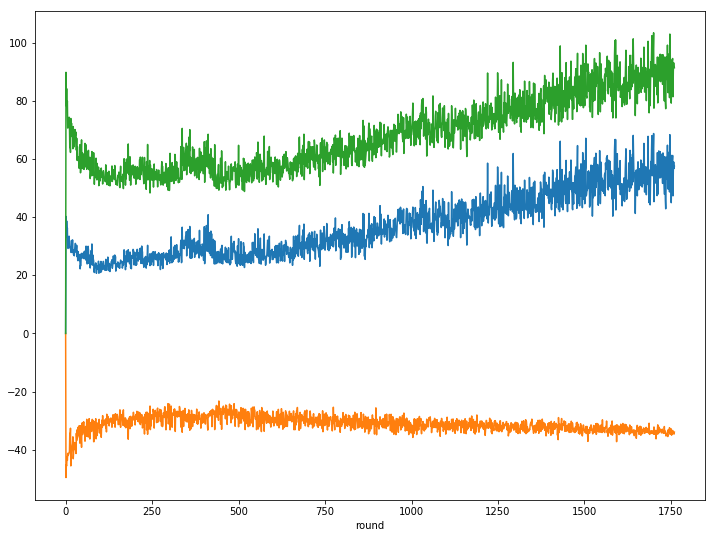
\includegraphics[width=\textwidth]{h1allgap.png}
\end{frame}

\begin{frame}
  \frametitle{Add-only Network Update Heuristic}
  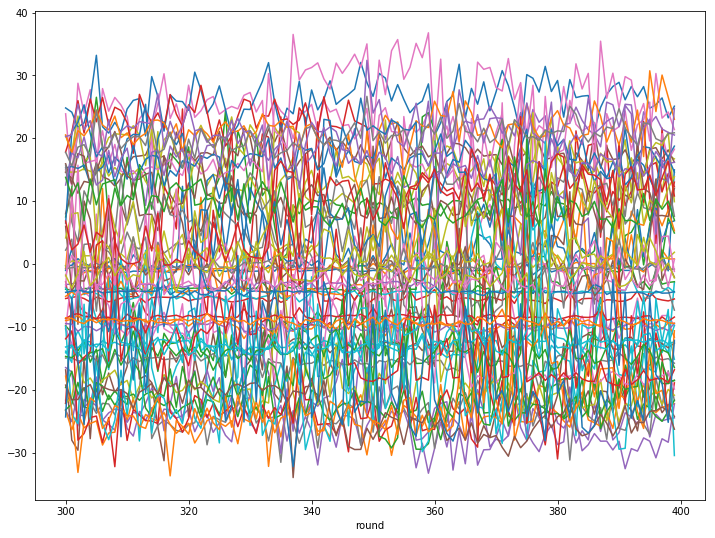
\includegraphics[width=\textwidth]{h1bestwealth.png}
\end{frame}

\begin{frame}
  \frametitle{Add-only Network Update Heuristic}
  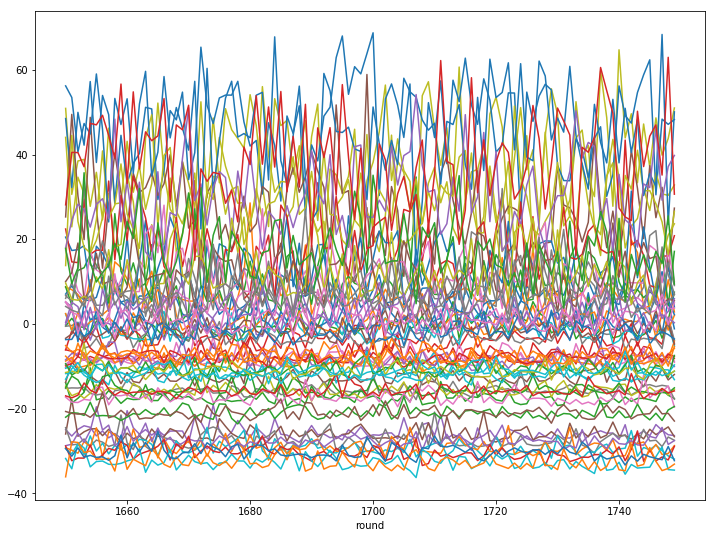
\includegraphics[width=\textwidth]{h1inequality.png}
\end{frame}

\begin{frame}
  \frametitle{Add-only Network Update Heuristic}
  \begin{itemize}
  \item Computationally expensive without parallelization
  \item Diverges with respect to wealth effect gap
  \item Finds price quickly
  \item Consistently reduces wealth effect in initial rounds
  \end{itemize}
\end{frame}

\begin{frame}
  \frametitle{Add-only Network Update Heuristic}
  At the end of each epoch:
  \begin{enumerate}
  \item Identify worst-off agent
  \item Add edge to random agent that is not already a neighbor
  \item Randomly remove an edge connecting agents that both have two or more neighbors
  \item Stop when graph is complete
  \end{enumerate}
\end{frame}

\begin{frame}
  \frametitle{Add-and-remove Network Update Heuristic}
  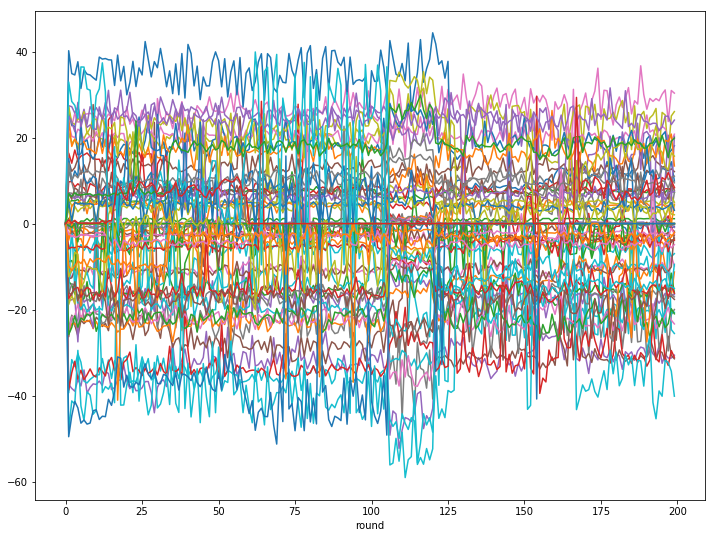
\includegraphics[width=\textwidth]{h2startwealth.png}
\end{frame}

\begin{frame}
  \frametitle{Add-and-remove Network Update Heuristic}
  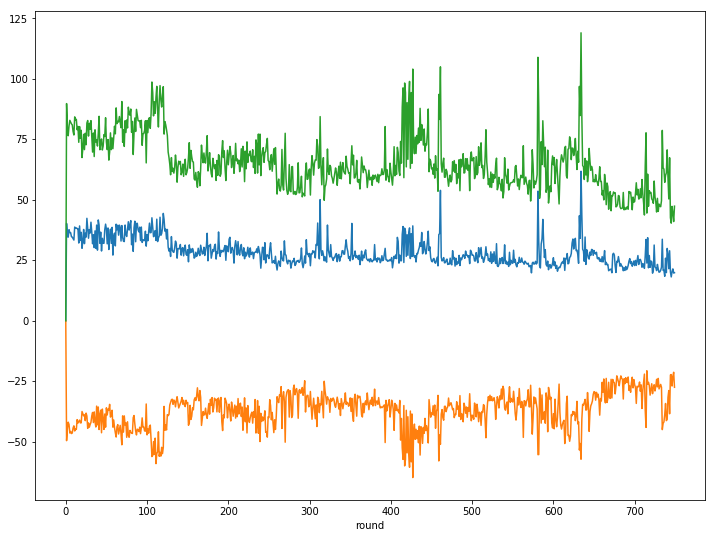
\includegraphics[width=\textwidth]{h2startgap.png}
\end{frame}

\begin{frame}
  \frametitle{Add-and-remove Network Update Heuristic}
  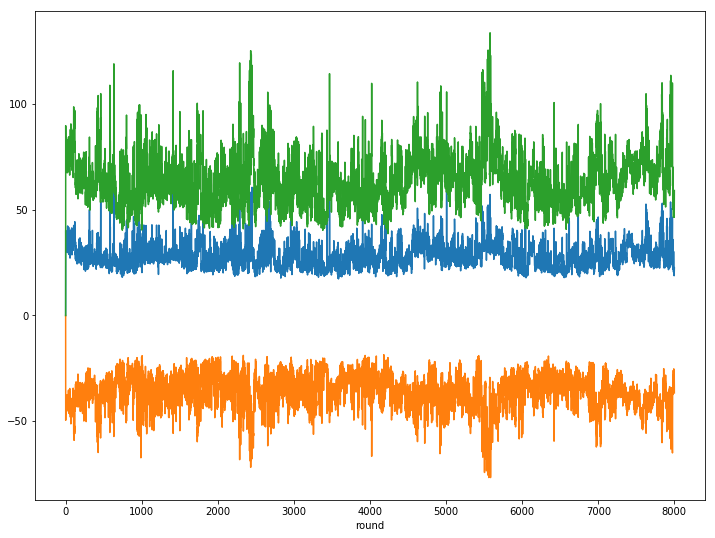
\includegraphics[width=\textwidth]{h2allgap.png}
\end{frame}

\begin{frame}
  \frametitle{Add-and-remove Network Update Heuristic}
  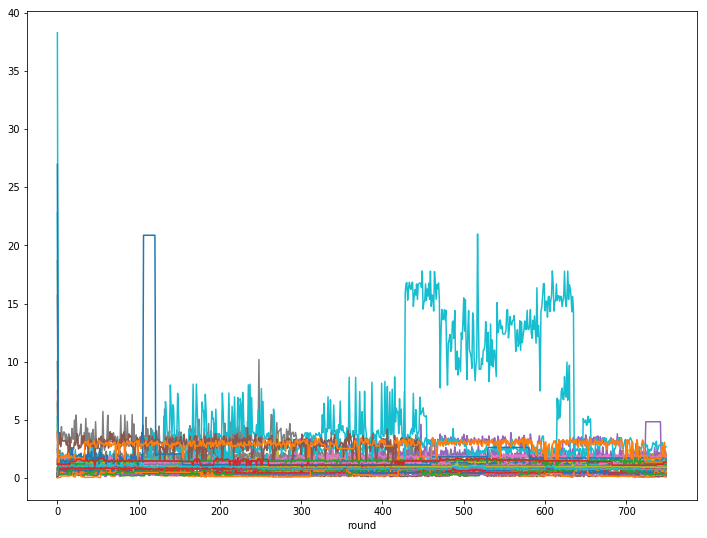
\includegraphics[width=\textwidth]{h2prices.png}
\end{frame}

\begin{frame}
  \frametitle{Add-and-remove Network Update Heuristic}
  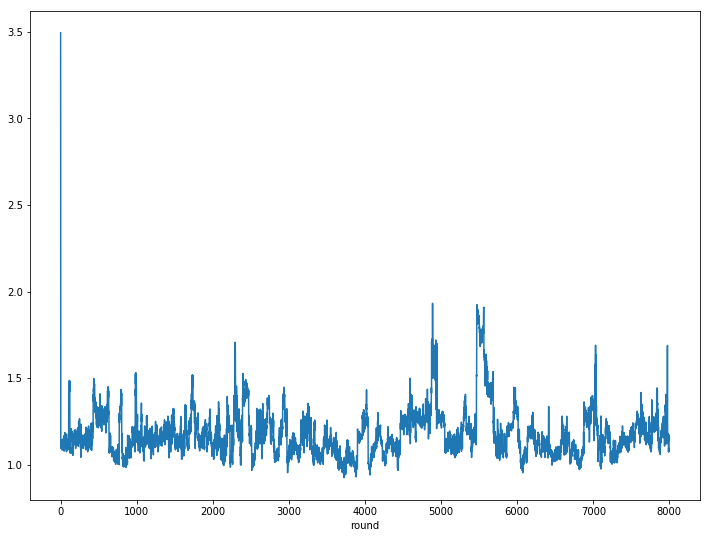
\includegraphics[width=\textwidth]{h2allpriceave.png}
\end{frame}

\begin{frame}
  \frametitle{Add-only Network Update Heuristic}
  \begin{itemize}
  \item More efficient per agent
  \item Better solution but convergence trend is not clear
  \item Price fluctuates
  \item Some agents do not trade
  \end{itemize}
\end{frame}

\begin{frame}
  \frametitle{Discussion}
  \begin{itemize}
    \item Some evidence that wealth effect and network topology can improve
      solutions
    \item Need to address non-trading/disconnected agents
    \item Need to implement parallel version
    \item Incorporate other data such as price and trade volume
    \item Other agent parameters
    \item More than two goods
  \end{itemize}
\end{frame}

\begin{frame}
  \frametitle{References}
  \bibliographystyle{plainnat}
  \bibliography{de.bib}
\end{frame}

\end{document}